\documentclass[10pt,aspectratio=169]{beamer}
\usepackage{tikz}
\usepackage[utf8]{inputenc}
\usepackage[english]{babel}
\usepackage{verbatim}
\usepackage{listings}
\usetikzlibrary{positioning}
\usetikzlibrary{arrows}

\lstset{
  language=C++,                 % the language of the code
  backgroundcolor=\color{white},   % choose the background color; you must add \usepackage{color} or \usepackage{xcolor}
  basicstyle=\ttfamily\footnotesize,        % the size of the fonts that are used for the code
  columns=fullflexible,
  breakatwhitespace=false,         % sets if automatic breaks should only happen at whitespace
  breaklines=true,                 % sets automatic line breaking
  keywordstyle=\color{blue!80!black},       % keyword style
  captionpos=b,                    % sets the caption-position to bottom
  commentstyle=\color{green!50!black},       % comment style
  deletekeywords={},            % if you want to delete keywords from the given language
  escapeinside={\%*}{*)},          % if you want to add LaTeX within your code
  extendedchars=true,              % lets you use non-ASCII characters; for 8-bits encodings only, does not work with UTF-8
  frame=no,                    % adds a frame around the code
  keepspaces=true,                 % keeps spaces in text, useful for keeping indentation of code (possibly needs columns=flexible)
  morekeywords={using, static_assert, uint8_t, uint16_t, uint32_t, size_t},            % if you want to add more keywords to the set
  numbers=none,                    % where to put the line-numbers; possible values are (none, left, right)
  numbersep=7pt,                   % how far the line-numbers are from the code
  numberstyle=\tiny\color{black}, % the style that is used for the line-numbers
  rulecolor=\color{black},         % if not set, the frame-color may be changed on line-breaks within not-black text (e.g. comments (green here))
  showspaces=false,                % show spaces everywhere adding particular underscores; it overrides 'showstringspaces'
  showstringspaces=false,          % underline spaces within strings only
  showtabs=false,                  % show tabs within strings adding particular underscores
  stepnumber=1,                    % the step between two line-numbers. If it's 1, each line will be numbered
  stringstyle=\color{red},     % string literal style
  tabsize=2,                       % sets default tabsize to 2 spaces
  title=\lstname                   % show the filename of files included with \lstinputlisting; also try caption instead of title
}

%\makeatletter
%\define@key{beamerframe}{t}[true]{% top
%\beamer@frametopskip=.2cm plus .5\paperheight\relax%
%\beamer@framebottomskip=0pt plus 1fill\relax%
%\beamer@frametopskipautobreak=\beamer@frametopskip\relax%
%\beamer@framebottomskipautobreak=\beamer@framebottomskip\relax%
%\def\beamer@initfirstlineunskip{}%
%}
%\makeatother   

%__________________________________________________________

% Possible themes

%\usetheme{AnnArbor}       % Bad color
%\usetheme{Antibes}       % Not good
%\usetheme{Bergen}        % Wastes space
%\usetheme{Berkeley}      % Very good
%\usetheme{Berlin}        % Very good
%\usetheme{Boadilla}      % Good
%\usetheme{CambridgeUS}   % Very good but no section list
%\usetheme{Copenhagen}    %  Limpo
%\usetheme{Dresden}       %  Vale a pena tambem
%\usetheme{Frankfurt}     % limpo, com lista mas sem pagina
%\usetheme{Goettingen}    % Lista de secoes na lateral esquerda
%\usetheme{Hannover}      %  Lista de secoes na lateral direita sem pagina
%\usetheme{Ilmenau}       % Com secao e sub
%\usetheme{JuanLesPins}   % Mais ou menos
%\usetheme{Luebeck}       % Limpo e bem organizado
\usetheme{Madrid}        % So titulo e com pagina
%\usetheme{Malmoe}        % Nao tem caixa para o titulo
%\usetheme{Marburg}       % Bem organizado, sem caixa pra titulo e com lista na direita
%\usetheme{Montpellier}   % Nao gosto do design
%\usetheme{PaloAlto}      % Boa escolha
%\usetheme{Pittsburgh}    % Fraco
%\usetheme{Rochester}     % So caixa pro titulo
%\usetheme{Singapore}     % Fraco
%\usetheme{Szeged}        % Legal
%\usetheme{Warsaw}        % Bom
%\usetheme{boxes}         % Fraco
%\usetheme{default}       % Fraco
%__________________________________________________________

% Possible color themes

%\usecolortheme{albatross}
%\usecolortheme{beaver}         % Acho que é esse.
%\usecolortheme{beetle}        % Bom mas escuro
%\usecolortheme{crane}         % muito boa    
%\usecolortheme{default}        
%\usecolortheme{dolphin}      
%\usecolortheme{dove}          % legal
%\usecolortheme{fly}    
%\usecolortheme{lily}       
\usecolortheme{orchid}       
%\usecolortheme{seagull}       % excelente mas cinza
%\usecolortheme{seahorse}     
%\usecolortheme{sidebartab}    
%\usecolortheme{whale}       
%\usecolortheme{wolverine}       

\colorlet{memC}{brown!70!black}
\colorlet{eleC}{orange!70!black}

\colorlet{alertc}{red!80!black}

\colorlet{arraycontc}{green!70!black}
\colorlet{nodecontc}{blue!70!black}
\colorlet{bothcontc}{orange!70!black}

\tikzstyle{mbu}=[draw,node distance=0cm, fill=memC,shape=rectangle,minimum height=0.5cm  ,minimum width=0.5cm  ,inner sep=1ex]
\tikzstyle{mbd}=[draw,node distance=0cm, fill=memC,shape=rectangle,minimum height=0.5cm  ,minimum width=1.0cm  ,inner sep=1ex]
\tikzstyle{mbq}=[draw,node distance=0cm, fill=memC,shape=rectangle,minimum height=0.5cm  ,minimum width=2.0cm  ,inner sep=1ex]
\tikzstyle{mbo}=[draw,node distance=0cm, fill=memC,shape=rectangle,minimum height=0.5cm  ,minimum width=4.0cm  ,inner sep=1ex]

\tikzstyle{ebu}=[draw,node distance=0cm, fill=eleC,shape=rectangle,minimum height=0.5cm  ,minimum width=0.5cm  ,inner sep=1ex]
\tikzstyle{ebd}=[draw,node distance=0cm, fill=eleC,shape=rectangle,minimum height=0.5cm  ,minimum width=1.0cm  ,inner sep=1ex]
\tikzstyle{ebq}=[draw,node distance=0cm, fill=eleC,shape=rectangle,minimum height=0.5cm  ,minimum width=2.0cm  ,inner sep=1ex]
\tikzstyle{ebo}=[draw,node distance=0cm, fill=eleC,shape=rectangle,minimum height=0.5cm  ,minimum width=4.0cm  ,inner sep=1ex]

\tikzstyle{lbu}=[node distance=0cm, shape=rectangle,minimum height=0.5cm, minimum width=0.5cm, inner sep=1ex]
\tikzstyle{lbd}=[node distance=0cm, shape=rectangle,minimum height=0.5cm, minimum width=1.0cm, inner sep=1ex]
\tikzstyle{lbq}=[node distance=0cm, shape=rectangle,minimum height=0.5cm, minimum width=2.0cm, inner sep=1ex]
\tikzstyle{lbo}=[node distance=0cm, shape=rectangle,minimum height=0.5cm, minimum width=4.0cm, inner sep=1ex]

\tikzstyle{marrow}=[very thick, densely dotted,>=stealth,->, color=black]
\tikzstyle{earrow}=[very thick, >=stealth,->, color=black]
\tikzstyle{rearrow}=[very thick, >=stealth,<-, color=black]

\def\mbu{\node[style=mbu]}
\def\mbd{\node[style=mbd]}
\def\mbq{\node[style=mbq]}
\def\mbo{\node[style=mbo]}
\def\ebu{\node[style=ebu]}
\def\ebd{\node[style=ebd]}
\def\ebq{\node[style=ebq]}
\def\ebo{\node[style=ebo]}

\def\lbu{\node[style=lbu]}
\def\lbd{\node[style=lbd]}
\def\lbq{\node[style=lbq]}
\def\lbo{\node[style=lbo]}

\def\marrow{\draw[style=marrow]}
\def\earrow{\draw[style=earrow]}
\def\rearrow{\draw[style=rearrow]}

%__________________________________________________________
% Apenas para o tema madrid

%\defbeamertemplate*{footline}{my infolines theme}
%{
%  \leavevmode%
%    \hbox{%
%      \begin{beamercolorbox}[wd=.333333\paperwidth,ht=2.25ex,dp=1ex,center]{author in head/foot}%
%        \usebeamerfont{author in head/foot}\insertshortauthor~~\insertshortinstitute
%        \end{beamercolorbox}%
%        \begin{beamercolorbox}[wd=.333333\paperwidth,ht=2.25ex,dp=1ex,center]{title in head/foot}%
%        \usebeamerfont{title in head/foot}\insertshorttitle
%        \end{beamercolorbox}%
%        \begin{beamercolorbox}[wd=.333333\paperwidth,ht=2.25ex,dp=1ex,right]{date in head/foot}%
%        \usebeamerfont{date in head/foot}\insertshortdate{}\hspace*{2em}
%      \insertframenumber{} / \inserttotalframenumber\hspace*{2ex}
%      \end{beamercolorbox}}%
%        \vskip0pt%
%}
%__________________________________________________________

\mode<presentation>
{
  %\setbeamercovered{transparent}
   %\setbeamertemplate{footline}[frame number]
  % or whatever (possibly just delete it)
}

\title[Node allocation in STL containers] {Node allocation in STL containers}

\subtitle[Improving the memory menagement] {Improving the memory menagement}

\author[Marcelo Zimbres] {Marcelo Zimbres}

\institute[Presentation to WG21-SG14]
{
}

\date[Magstadt - Germany] {}

\subject{Node allocation 3}

% If you have a file called "university-logo-filename.xxx", where xxx
% is a graphic format that can be processed by latex or pdflatex,
% resp., then you can add a logo as follows:

%\pgfdeclareimage[height=1.2cm]{Wavelet}{fig/skymapJ8j2N127.pdf}
%\logo{\pgfuseimage{Wavelet}}

% Delete this, if you do not want the table of contents to pop up at
% the beginning of each subsection:
%\AtBeginSubsection[]
%{
%  \begin{frame}<beamer>{Outline}
%    %\tableofcontents[currentsection,currentsubsection]
%    \tableofcontents
%  \end{frame}
%}

% If you wish to uncover everything in a step-wise fashion, uncomment
% the following command: 

%\beamerdefaultoverlayspecification{<+->}

\begin{document}

%____________________________________________________________
\begin{frame}
  \titlepage
\end{frame}

%____________________________________________________________
%\begin{frame}{Outline}
%  \tableofcontents[pausesections]
%  % You might wish to add the option [pausesections]
%\end{frame}

%____________________________________________________________
%\begin{frame}<beamer>{Outline}
%   \tableofcontents[currentsection,currentsubsection]
%\end{frame}


% Since this a solution template for a generic talk, very little can
% be said about how it should be structured. However, the talk length
% of between 15min and 45min and the theme suggest that you stick to
% the following rules:  

% - Exactly two or three sections (other than the summary).
% - At *most* three subsections per section.
% - Talk about 30s to 2min per frame. So there should be between about
%   15 and 30 frames, all told.

%____________________________________________________________
\begin{frame}{Goals - Target audience}{}
\begin{columns}
\begin{column}{0.50\textwidth}
\begin{block} {Goals}
\begin{itemize}
    \item Provide building blocks for memory allocation.
    \item Profit from static type information.
    \item Reduce pointer overhead in nodes.
    \item Alternative to pointer chasing on traversal.
    \item Allow fine tunning and reduce complexity.
    \item Reduce centralization.
\end{itemize}
\end{block}

\end{column}

\begin{column}{0.35\textwidth}
\begin{block} {Target audience}
\begin{itemize}
    \item Embedded developers.
    \item Resource constrained systems.
    \item High performace.
    \item 24/7 availability.
\end{itemize}
\end{block}
\end{column}
\end{columns}
\end{frame}

%____________________________________________________________
\begin{frame}{Outline}
   %\tableofcontents[currentsection,currentsubsection]
   \tableofcontents
\end{frame}

\section{STL and memory management}

\subsection{Dynamic memory allocations in \texttt{C++}}

%____________________________________________________________
\begin{frame}[fragile]{Memory allocation in \texttt{C++}}
{Note: I will use {\it Heap} to refer to free storage memory.}
\begin{columns}
\begin{column}[t]{0.45\textwidth}
\begin{block}{Memory segments}
\begin{itemize}
\item Data: Global and static variables.
\item Stack: Restricted lifetime, small.
\item Heap: No restriction on lifetime and size.
\end{itemize}
\end{block}
%\vspace{0.5cm}
\begin{lstlisting}
// Allocation in the data segment.
static int a; // Deallocation at programm exit

// Allocation in the function stack frame.
int b; // Deallocation upon funtion return.

// Dynamic allocation on the heap.
auto* p = new int;

delete p; // Deallocation is not automatic.
\end{lstlisting}
\end{column}

\begin{column}[t]{0.45\textwidth}
\begin{block}{Inside STL containers}
\begin{itemize}
\item Idea of segments abstracted away.
\item Memory requested from allocators.
\item Provide a customization point.
\end{itemize}
\end{block}
%\vspace{0.5cm}
\begin{lstlisting}
std::allocator<int> alloc; // Can have state.

// Requests enough space for one int.
auto* p = alloc.allocate(1);

// Returns memory to the allocator.
alloc.deallocate(p, 1);

// See also std::allocator_traits.
\end{lstlisting}
\end{column}
\end{columns}
\end{frame}

%____________________________________________________________
\begin{frame}[fragile]
{Definitions (in the context of STL containers)}
\begin{columns}
\begin{column}{0.45\textwidth}

\begin{block} {Node allocation}
I will use {\bf \color{alertc} node allocation} to refer to
allocations that have always the same size.
\end{block}
\vspace{0.5cm}
\begin{lstlisting}
// Allocations inside std::list are one
// element at time (constant size).
auto* p1 = alloc.allocate(1);
auto* p2 = alloc.allocate(1);
auto* p3 = alloc.allocate(1);
auto* p4 = alloc.allocate(1);
\end{lstlisting}

\end{column}

\begin{column}{0.45\textwidth}
\begin{block} {Array allocation}
For allocations with varying sizes I will use the term {\bf \color{alertc} array allocation}.
\end{block}
\vspace{0.5cm}
\begin{lstlisting}
// Allocations inside std::vector have
// increasing sizes (e.g. push_back).
auto* p1 = alloc.allocate(2);
auto* p2 = alloc.allocate(4);
auto* p3 = alloc.allocate(8);
auto* p4 = alloc.allocate(16);
\end{lstlisting}
\end{column}
\end{columns}
\end{frame}

\subsection{Allocation patterns}

\begin{frame}{Containers and their allocation patterns}
\begin{columns}
\begin{column}[c]{0.45\textwidth}

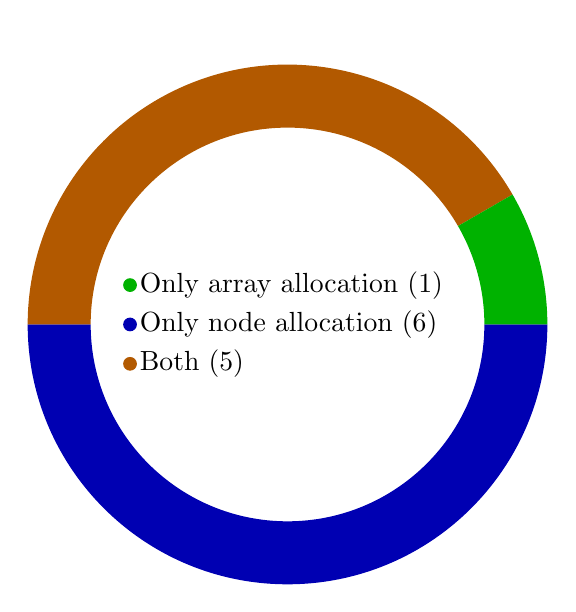
\begin{tikzpicture}[scale=1.0]
\fill[nodecontc]  (180:2.5cm) -- (180: 3.3cm) arc (180:360:3.3cm) -- (360:2.5cm) arc (360:180:2.5cm);
\fill[bothcontc]   (30:2.5cm) -- (30:3.3cm) arc (30:180:3.3cm)  -- (180:2.5cm) arc (180:30:2.5cm);
\fill[arraycontc] (0:2.5cm) -- (0:3.3cm) arc (0:30:3.3cm) -- (30:2.5cm) arc (30:0:2.5cm);

\filldraw[arraycontc] (-2cm,0.5cm) circle (0.08cm) node[right] {\color{black}Only array allocation (1)};
\filldraw[nodecontc] (-2cm,0.0cm) circle (0.08cm) node[right] {\color{black}Only node allocation (6)};
\filldraw[bothcontc] (-2cm,-0.5cm) circle (0.08cm) node[right] {\color{black}Both (5)};
\end{tikzpicture}
\end{column}

\begin{column}[c]{0.45\textwidth}
\begin{block} {STL containers (12)}
\begin{itemize}
\item \texttt{\color{arraycontc} std::vector}
\item \texttt{\color{nodecontc} std::list}
\item \texttt{\color{nodecontc} std::forward\_list}
\item \texttt{\color{nodecontc} std::set}
\item \texttt{\color{nodecontc} std::multiset}
\item \texttt{\color{nodecontc} std::map}
\item \texttt{\color{nodecontc} std::multimap}
\item \texttt{\color{bothcontc} std::deque}
\item \texttt{\color{bothcontc} std::unordered\_set}
\item \texttt{\color{bothcontc} std::unordered\_multiset}
\item \texttt{\color{bothcontc} std::unordered\_map}
\item \texttt{\color{bothcontc} std::unordered\_multimap}
\end{itemize}
\end{block}
\end{column}

\end{columns}
\end{frame}

%___________________________________________________________
\begin{frame}{Node allocation in the STL matters}

\begin{columns}
\begin{column}[c]{0.45\textwidth}
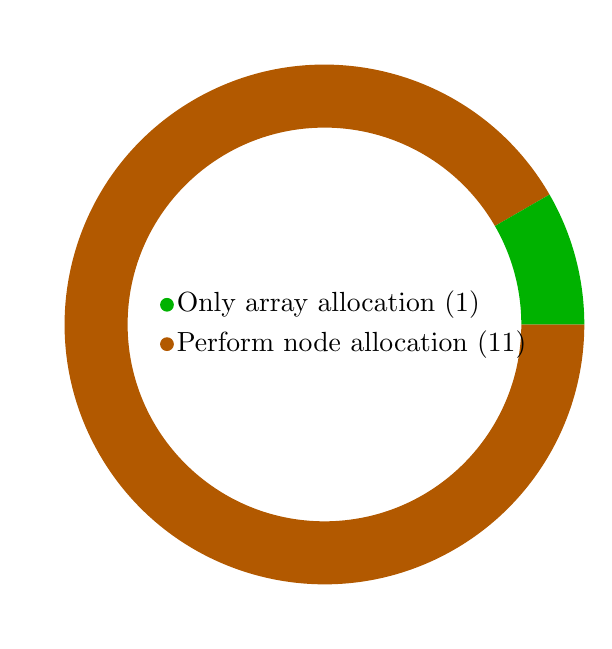
\begin{tikzpicture}[scale=1.0]
\fill[bothcontc]  (30:2.5cm) -- (30:3.3cm) arc (30:360:3.3cm) -- (360:2.5cm) arc (360:30:2.5cm);
\fill[arraycontc] (0:2.5cm) -- (0:3.3cm) arc (0:30:3.3cm) -- (30:2.5cm) arc (30:0:2.5cm);

\filldraw[arraycontc] (-2cm,0.25cm) circle (0.08cm) node[right] {\color{black} Only array allocation (1)};
\filldraw[bothcontc] (-2cm,-0.25cm) circle (0.08cm) node[right] {\color{black} Perform node allocation (11)};
\end{tikzpicture}
\end{column}

\begin{column}[c]{0.45\textwidth}
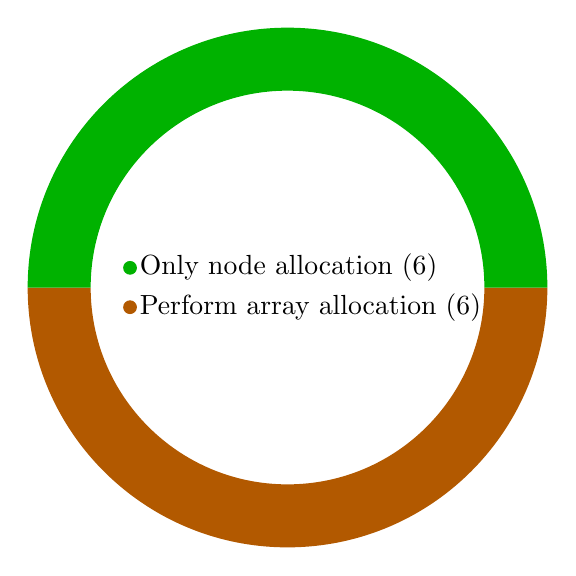
\begin{tikzpicture}[scale=1.0]
\fill[bothcontc]  (180:2.5cm) -- (180:3.3cm) arc (180:360:3.3cm) -- (360:2.5cm) arc (360:180:2.5cm);
\fill[arraycontc] (0:2.5cm) -- (0:3.3cm) arc (0:180:3.3cm) -- (180:2.5cm) arc (180:0:2.5cm);

\filldraw[arraycontc] (-2cm,0.25cm) circle (0.08cm) node[right] {\color{black} Only node allocation (6)};
\filldraw[bothcontc] (-2cm,-0.25cm) circle (0.08cm) node[right] {\color{black} Perform array allocation (6)};
\end{tikzpicture}
\end{column}
\end{columns}
\end{frame}

%____________________________________________________________
\begin{frame}[fragile]
{Why the current allocator interface is suboptimal}
{A closer look at allocators}
\begin{columns}
\begin{column}{0.35\textwidth}

%\begin{block} {\texttt{allocate(n)}}
%\end{block}
\begin{lstlisting}
pointer allocate(size_type n, ...);



void deallocate( pointer p
               , size_type n);
\end{lstlisting}

\end{column}

\begin{column}{0.55\textwidth}
\begin{block} {Allocators and size management}
\begin{itemize}
\item Allocation size is a runtime variable.
\item Node allocation is however known at compile time.
\item Blesses array allocation. Unaware of node allocation.
\item No simple implementation. Has to handle any sizes.
\item Leads to overly complex strategies.
\item Leads to overheads like bookkeeping information.
\item Encourages centralization.
\end{itemize}

\end{block}

\end{column}
\end{columns}
\end{frame}
%____________________________________________________________
\begin{frame}[t]{Node allocation illustration}
{How it is implemented in practice: pooling}
\begin{block} {Procedure}
\begin{enumerate}
\item<alert@1> Get a continuos block of memory with enough space for $n$ nodes.
\item<alert@2> Divide in blocks, link them as a stack and repeat if ever run out of memory.
\item<alert@6> After some allocations and deallocations.
\end{enumerate}
\end{block}

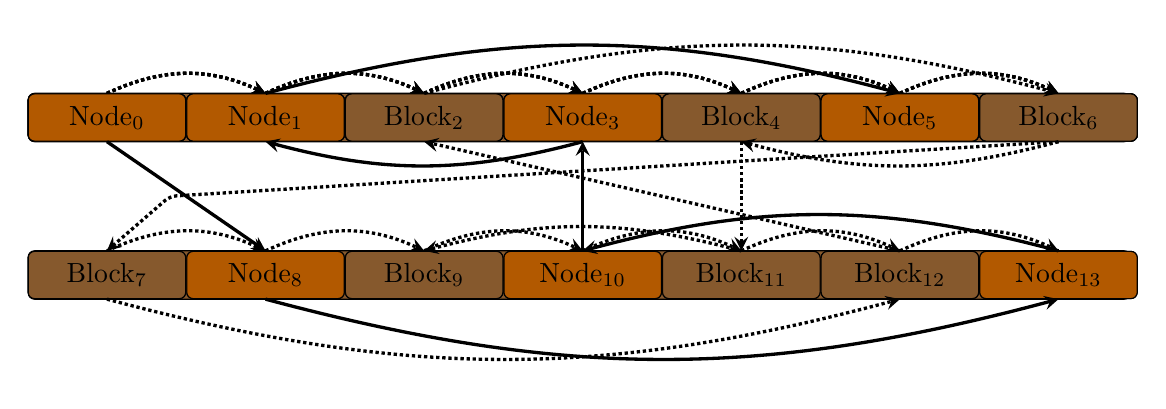
\begin{tikzpicture}[scale=1.0, rounded corners=0.8mm]

   \uncover<1> {
      \node[draw, node distance=0cm, fill=memC, shape=rectangle,minimum height=0.5cm  ,minimum width=14.0cm  ,inner sep=1ex]
      (block) at (1cm, 4cm) {Block with enough space for $n$ nodes};
   }

   \uncover<2> {
      \mbq (node0)  at (-5.0,4.0) {Block$_0$};
      \mbq (node1)  [right=of node0] {Block$_1$};
      \mbq (node2)  [right=of node1] {Block$_2$};
      \mbq (node3)  [right=of node2] {Block$_3$};
      \mbq (node4)  [right=of node3] {Block$_4$};
      \mbq (node5)  [right=of node4] {Block$_5$};
      \mbq (node6)  [right=of node5] {Block$_6$};
   }

   \uncover<3> {
      \mbq (node0)  at (-5.0,4.0) {Block$_0$};
      \mbq (node1)  [right=of node0] {Block$_1$};
      \mbq (node2)  [right=of node1] {Block$_2$};
      \mbq (node3)  [right=of node2] {Block$_3$};
      \mbq (node4)  [right=of node3] {Block$_4$};
      \mbq (node5)  [right=of node4] {Block$_5$};
      \mbq (node6)  [right=of node5] {Block$_6$};

      \marrow (node0.north) to [bend right=-25] (node1.north);
      \marrow (node1.north) to [bend right=-25] (node2.north);
      \marrow (node2.north) to [bend right=-25] (node3.north);
      \marrow (node3.north) to [bend right=-25] (node4.north);
      \marrow (node4.north) to [bend right=-25] (node5.north);
      \marrow (node5.north) to [bend right=-25] (node6.north);
   }

   \uncover<4> {
      \mbq (node0)  at (-5.0,4.0) {Block$_0$};
      \mbq (node1)  [right=of node0] {Block$_1$};
      \mbq (node2)  [right=of node1] {Block$_2$};
      \mbq (node3)  [right=of node2] {Block$_3$};
      \mbq (node4)  [right=of node3] {Block$_4$};
      \mbq (node5)  [right=of node4] {Block$_5$};
      \mbq (node6)  [right=of node5] {Block$_6$};

      \marrow (node0.north) to [bend right=-25] (node1.north);
      \marrow (node1.north) to [bend right=-25] (node2.north);
      \marrow (node2.north) to [bend right=-25] (node3.north);
      \marrow (node3.north) to [bend right=-25] (node4.north);
      \marrow (node4.north) to [bend right=-25] (node5.north);
      \marrow (node5.north) to [bend right=-25] (node6.north);

      \node[draw, node distance=0cm, fill=memC, shape=rectangle,minimum height=0.5cm  ,minimum width=14.0cm  ,inner sep=1ex]
      (block) at (1cm, 2cm) {Run out of memory, get another block. };
   }

   \uncover<5> {
      \mbq (node0)  at (-5.0,4.0) {Block$_0$};
      \mbq (node1)  [right=of node0] {Block$_1$};
      \mbq (node2)  [right=of node1] {Block$_2$};
      \mbq (node3)  [right=of node2] {Block$_3$};
      \mbq (node4)  [right=of node3] {Block$_4$};
      \mbq (node5)  [right=of node4] {Block$_5$};
      \mbq (node6)  [right=of node5] {Block$_6$};

      \mbq (node7)  at (-5.0,2.0)     {Block$_7$};
      \mbq (node8)  [right=of node7] {Block$_8$};
      \mbq (node9)  [right=of node8] {Block$_9$};
      \mbq (node10) [right=of node9] {Block$_{10}$};
      \mbq (node11) [right=of node10] {Block$_{11}$};
      \mbq (node12) [right=of node11] {Block$_{12}$};
      \mbq (node13) [right=of node12] {Block$_{13}$};

      \marrow (node0.north) to [bend right=-25] (node1.north);
      \marrow (node1.north) to [bend right=-25] (node2.north);
      \marrow (node2.north) to [bend right=-25] (node3.north);
      \marrow (node3.north) to [bend right=-25] (node4.north);
      \marrow (node4.north) to [bend right=-25] (node5.north);
      \marrow (node5.north) to [bend right=-25] (node6.north);

      \marrow (node6.south)  -- (-4.2, 3.0) -- (node7.north);
      \marrow (node7.north)  to [bend right=-25] (node8.north);
      \marrow (node8.north)  to [bend right=-25] (node9.north);
      \marrow (node9.north)  to [bend right=-25] (node10.north);
      \marrow (node10.north) to [bend right=-25] (node11.north);
      \marrow (node11.north) to [bend right=-25] (node12.north);
      \marrow (node12.north) to [bend right=-25] (node13.north);
   }

   \uncover<6-> {
      \ebq (node0)  at (-5.0,4.0) {Node$_0$};
      \ebq (node1)  [right=of node0] {Node$_1$};
      \mbq (node2)  [right=of node1] {Block$_2$};
      \ebq (node3)  [right=of node2] {Node$_3$};
      \mbq (node4)  [right=of node3] {Block$_4$};
      \ebq (node5)  [right=of node4] {Node$_5$};
      \mbq (node6)  [right=of node5] {Block$_6$};

      \mbq (node7)  at (-5.0,2.0)     {Block$_7$};
      \ebq (node8)  [right=of node7] {Node$_8$};
      \mbq (node9)  [right=of node8] {Block$_9$};
      \ebq (node10) [right=of node9] {Node$_{10}$};
      \mbq (node11) [right=of node10] {Block$_{11}$};
      \mbq (node12) [right=of node11] {Block$_{12}$};
      \ebq (node13) [right=of node12] {Node$_{13}$};
   }

   \uncover<6-> {
      \earrow (node0.south) -- (node8.north);
      \earrow (node1.north) to [bend right=-15] (node5.north);
      \earrow (node3.south) to [bend right=-15] (node1.south);
      \earrow (node8.south) to [bend right=15] (node13.south);
      \earrow (node10.north) -- (node3.south);
      \earrow (node13.north) to [bend right=15] (node10.north);
   }

   \uncover<6-> {
      \marrow (node2.north) to [bend right=-15] (node6.north);
      \marrow (node6.south) to [bend right=-15] (node4.south);
      \marrow (node4.south) -- (node11.north);
      \marrow (node11.north) to [bend right=15] (node9.north);
      \marrow (node7.south) to [bend right=15] (node12.south);
      \marrow (node12.north) -- (node2.south);
   }

\end{tikzpicture}

\end{frame}

%____________________________________________________________
\begin{frame}[fragile]
{Simplicity matters}
{How node allocation is implemented}

\begin{columns}
\begin{column}{0.47\textwidth}
\begin{lstlisting}
pointer allocate_node()
{
 pointer q = avail; // The next free node
 if (avail)
   avail = avail->next;

 return q;
}

void deallocate_node(pointer p)
{
 p->next = avail;
 avail = p;
}
\end{lstlisting}
\end{column}
\begin{column}{0.47\textwidth}
\begin{block} {Clear behaviour}
Once you have nodes linked as a stack, allocation and
deallocation reduces to these functions.
\end{block}
\begin{lstlisting}
// Boost interface. Allows choosing the number
// of nodes per blocks. You know its best value
// better than malloc.
node_allocator< int
              , 256 // Nodes per block
              > alloc;
\end{lstlisting}
\end{column}
\end{columns}
\end{frame}

\subsection{Typical allocation goals and strategies}

%____________________________________________________________
\begin{frame}{Outline}
   \tableofcontents[currentsection,currentsubsection]
\end{frame}

%____________________________________________________________
\begin{frame}{Typical allocation goals and strategies}
{\texttt{malloc}, \texttt{jemalloc}, \texttt{tcmalloc},
\texttt{nedmalloc}, \texttt{hoard}, etc.}
\begin{columns}
\begin{column}{0.47\textwidth}
\begin{block} {Typical goals and strategies}
\begin{itemize}
\item Different strategy for small and big sizes.
\item Small sizes: Many pre-allocated blocks.
\item Large sizes: Best fit, rounding on memory pages.
\item Avoid fragmentation. Improve locality.
\item Avoid serialization on cuncurrent calls.
\item Thread local buffers.
\item Bookkeeping information on blocks.
\item Rounding allocation sizes to fit pre-allocated buffers.
\item Surprizing (upsetting) behaviour.
\end{itemize}
\end{block}
\end{column}

\begin{column}{0.47\textwidth}
\begin{block} {Centralization is bad}
\begin{itemize}
\item Which strategy is better for my use case?
\item Bookkeeping information, rounding, size management
are unnecessary on node allocation
\item Unclear behaviour for long running programms.
\item Compile time information should not be thrown away.
\item<alert@1> Node allocation is a building block.
\end{itemize}
\end{block}

\end{column}
\end{columns}
\end{frame}

%____________________________________________________________
\begin{frame}
{Surprises in allocator behaviour}
{Benchmarking \texttt{std::unordered\_set} with well known allocators}
\begin{columns}

    \begin{column}{0.47\textwidth}
        \begin{center}
            
            \includegraphics[scale=0.7]{fig/unordered_set_with_frag.pdf} \\
        \end{center}
    \end{column}

    \begin{column}{0.47\textwidth}
         \begin{block}{Why \texttt{std::allocator} performs poorly?}
           \begin{itemize}
           \item Difficult to say.
           \item Bookkeeping fields is making nodes bigger?
           \item Unoptimaly rounding and size management? 
           \item Should perform the same had node
           allocation been used internally.
           \item Scenario: Messy heap.
           \item {\color{alertc}This is unacceptable behaviour on many systems.}
           \end{itemize}
         \end{block}
    %    \texttt{std::set}
    %    \begin{center}
    %        \includegraphics[scale=0.6]{fig/set_bench.pdf} \\
    %    \end{center}
    \end{column}

\end{columns}
\end{frame}


%\subsection{Node allocation as a building block}

%___________________________________________________________________
\begin{frame}[t]{Pools of blocks with different sizes}
\begin{block}{Should not need this if compile time information had been used.}
\begin{itemize}
\item Many pre-allocated sizes. Possibly thread local.
\item Small sizes are rounded to one of these.
\item \texttt{std::malloc} has up to 170 of these lists.
\end{itemize}
\end{block}
\vspace{0.5cm}
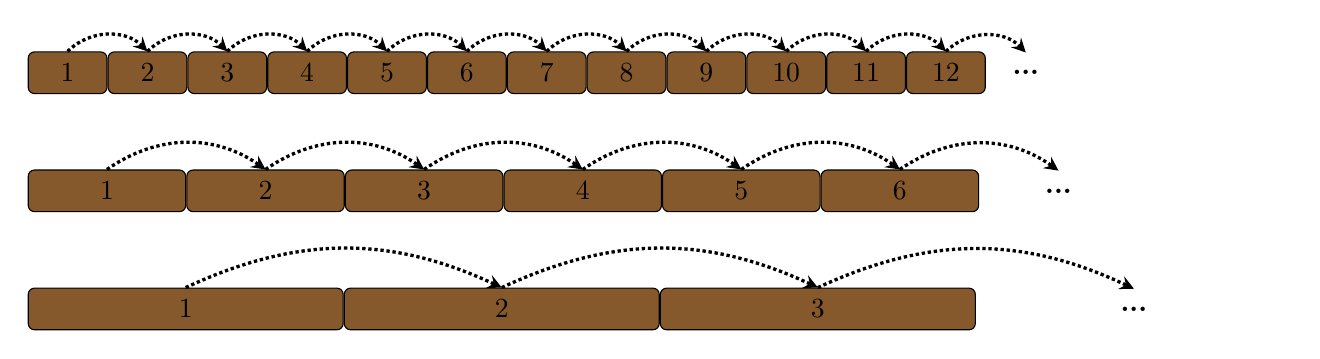
\begin{tikzpicture}[scale=1.0, rounded corners=0.8mm]
      % next
      \mbd (Unode0) at  (0.5,2.0)       {1};
      \mbd (Unode1)  [right=of Unode0]  {2};
      \mbd (Unode2)  [right=of Unode1]  {3};
      \mbd (Unode3)  [right=of Unode2]  {4};
      \mbd (Unode4)  [right=of Unode3]  {5};
      \mbd (Unode5)  [right=of Unode4]  {6};
      \mbd (Unode6)  [right=of Unode5]  {7};
      \mbd (Unode7)  [right=of Unode6]  {8};
      \mbd (Unode8)  [right=of Unode7]  {9};
      \mbd (Unode9)  [right=of Unode8]  {10};
      \mbd (Unode10) [right=of Unode9]  {11};
      \mbd (Unode11) [right=of Unode10] {12};
      \lbd (Unode12) [right=of Unode11] {\bf ...};

      \marrow (Unode0.north) to  [bend right=-45] (Unode1.north);
      \marrow (Unode1.north) to  [bend right=-45] (Unode2.north);
      \marrow (Unode2.north) to  [bend right=-45] (Unode3.north);
      \marrow (Unode3.north) to  [bend right=-45] (Unode4.north);
      \marrow (Unode4.north) to  [bend right=-45] (Unode5.north);
      \marrow (Unode5.north) to  [bend right=-45] (Unode6.north);
      \marrow (Unode6.north) to  [bend right=-45] (Unode7.north);
      \marrow (Unode7.north) to  [bend right=-45] (Unode8.north);
      \marrow (Unode8.north) to  [bend right=-45] (Unode9.north);
      \marrow (Unode9.north) to  [bend right=-45] (Unode10.north);
      \marrow (Unode10.north) to [bend right=-45] (Unode11.north);
      \marrow (Unode11.north) to [bend right=-45] (Unode12.north);
      % next
      \mbq (Qnode0) at  (1.0,0.5)      {1};
      \mbq (Qnode1)  [right=of Qnode0] {2};
      \mbq (Qnode2)  [right=of Qnode1] {3};
      \mbq (Qnode3)  [right=of Qnode2] {4};
      \mbq (Qnode4)  [right=of Qnode3] {5};
      \mbq (Qnode5)  [right=of Qnode4] {6};
      \lbq (Qnode6)  [right=of Qnode5] {\bf ...};

      \marrow (Qnode0.north) to  [bend right=-35] (Qnode1.north);
      \marrow (Qnode1.north) to  [bend right=-35] (Qnode2.north);
      \marrow (Qnode2.north) to  [bend right=-35] (Qnode3.north);
      \marrow (Qnode3.north) to  [bend right=-35] (Qnode4.north);
      \marrow (Qnode4.north) to  [bend right=-35] (Qnode5.north);
      \marrow (Qnode5.north) to  [bend right=-35] (Qnode6.north);
      % next
      \mbo (Onode0) at  (2.0,-1.0)     {1};
      \mbo (Onode1)  [right=of Onode0] {2};
      \mbo (Onode2)  [right=of Onode1] {3};
      \lbo (Onode3)  [right=of Onode2] {\bf ...};

      \marrow (Onode0.north) to [bend right=-25] (Onode1.north);
      \marrow (Onode1.north) to [bend right=-25] (Onode2.north);
      \marrow (Onode2.north) to [bend right=-25] (Onode3.north);

\end{tikzpicture}
\end{frame}

%____________________________________________________________
\begin{frame}[fragile]
{}

\begin{columns}
\begin{column}{0.10\textwidth}
\end{column}
\begin{column}{0.80\textwidth}
\begin{block}{Node allocation is a building block}
  I've been arguing that node allocation is an important concept and deserves
  proper support in the STL. Now lets us see how to do it and what further
  benefits it brings.
\end{block}
\end{column}
\begin{column}{0.10\textwidth}
\end{column}
\end{columns}
\end{frame}

\section{Supporting node-allocation in the STL}

%____________________________________________________________
\begin{frame}{Outline}
   \tableofcontents[currentsection,currentsubsection]
\end{frame}

\subsection{Proposal}

%____________________________________________________________
\begin{frame}{Should node allocation be standardized}{Proposal to the ISO \texttt{C++} Standards Committee}
\vspace{-3cm}
    \begin{center}
        \includegraphics[scale=0.6]{fig/prop1.pdf} \\
    \end{center}
\end{frame}

%____________________________________________________________
\begin{frame}[fragile]
{Node allocation support}
{Two new member functions and one typedef in \texttt{std::allocator\_traits}}

\begin{columns}
\begin{column}{0.60\textwidth}
\begin{lstlisting}
// Boost interface (thanks to Ion Gaztanaga for
// suggesting it).
template<class Alloc>
struct allocator_traits {
  // Calls a.allocate_node() if present otherwise calls
  // Alloc::allocate(1). Memory allocated with this
  // function must be deallocated with deallocate_node.
  pointer allocate_node(Alloc& a);

  // Calls a.deallocate_node(pointer) if present
  // otherwise calls Alloc::deallocate(p, 1). Can only
  // be used with memory allocated with allocate_node.
  void deallocate_node(Alloc& a, pointer p);
};
\end{lstlisting}
\end{column}

\begin{column}{0.40\textwidth}
\begin{block}{Why}
\begin{itemize}
\item No size menagement.
\item Well defined behaviour.
\item Names reflects intension.
\item {\color{alertc}No surprises}
\end{itemize}
\end{block}
\end{column}

\end{columns}

\end{frame}

%____________________________________________________________
\begin{frame}[fragile]
{Containers that perform both {\it node} and {\it array} allocation}
{Exposing the node type}

\begin{columns}
\begin{column}[t]{0.47\textwidth}
\begin{block}{Problem}
Which allocator is the node allocator?
\end{block}
\begin{lstlisting}
// Allocator instance does not know which
// type it will serve.
my_alloc<int> alloc;

// Rebinds to two further allocator types
// and construct them from alloc.
std::unordered_set< int, ...
                  , my_alloc<int>> obj(alloc);

// Triggers both node and array allocation.
// Which allocator will have n = 1 is unknown.
obj.insert(10);
\end{lstlisting}
\end{column}
\begin{column}[t]{0.47\textwidth}
\begin{block}{Fix}
Let the allocator know the node type.
\end{block}
\begin{lstlisting}
using node_type =
    std::unordered_set<int>::node_type

// Allocator knows the node type and offers
// only allocate_node().
my_alloc<int, node_type> alloc;

std::unordered_set< int
                  , my_alloc<int, node_type>
                  > obj(alloc);

// No need of testing n == 1. 
obj.insert(10);
\end{lstlisting}
\end{column}
\end{columns}

\end{frame}

%____________________________________________________________
\begin{frame}[fragile]
{The node type is not independent of the allocator}
{Fancy pointers}

\begin{columns}
\begin{column}[t]{0.47\textwidth}
\begin{block}{Typical node}
No customization of the pointer type.
\end{block}
\begin{lstlisting}
template <class T>
struct node {
  T info;
  node* next;
};
\end{lstlisting}
\end{column}
\begin{column}[t]{0.47\textwidth}
\begin{block}{STL node}
Allows customization of the pointer type.
\end{block}
\begin{lstlisting}
template < class T
         , class Ptr // Defined by the allocator
         >
struct node {
  T info;
  using pointer = typename
      std::pointer_traits<Ptr>::template
          rebind<node<T, Ptr>>;
  pointer next;
};
\end{lstlisting}
\end{column}
\end{columns}
\end{frame}

%____________________________________________________________
\begin{frame}[fragile]
{We need to rebind the node type}
{Node interface}

\begin{block}{Recursive problem}
\begin{itemize}
\item The node type is unknown until the container type is known.
\item The allocator type is needed to define the container.
\item The allocator type needs the node type to be defined.
\item {\color{alertc}Solution: Offer a rebind function.}
\end{itemize}
\end{block}

\begin{columns}
\begin{column}[t]{0.47\textwidth}
\begin{lstlisting}
// Rebinding allows changing the node pointer
// type. Allocator uses it to define the node
// with its own pointer type.
template <class T, class Ptr>
struct node {
  ...
  template<class U, class K>
  struct rebind { using other = node<U , K>; };
};

\end{lstlisting}

\end{column}

\begin{column}[t]{0.47\textwidth}
\begin{lstlisting}
// Gets the node type with any allocator.
using node_type = typename
    std::list<int>::node_type.

// Allocator rebinds the node type internally.
// to whatever pointer type it uses.
my_alloc<int, node_type> alloc;
\end{lstlisting}
\end{column}
\end{columns}
\end{frame}

%____________________________________________________________
\begin{frame}[fragile]
{Simple use case}
{Containers with small number of elements}

\begin{columns}
\begin{column}[t]{0.47\textwidth}
\begin{lstlisting}
std::aligned_storage< sizeof(node_type)
                    , alignof(node_type)
                    >::type buffer[64];

// Allocator with very simple implementation.
node_allocator< int, node_type
              , 64> alloc(buffer);

std::list< int , alloc_type<int, node_type>
         > l(alloc);

// Allocation and deallocation implemented
// with 6 lines of code.
l = {27, 1, 60};
\end{lstlisting}
\end{column}
\begin{column}[t]{0.47\textwidth}
\begin{block}{Thoughts}
\begin{itemize}
\item Node sizes are known at compile time.
\item Stores them in the stack.
\item Minimum amount of memory needed for $n$ elements.
\item Never touches the heap.
\item {\color{alertc}Let us move to more interesting usages.}
\end{itemize}
\end{block}
\end{column}
\end{columns}
\end{frame}

\subsection{Traversal without pointer chasing}

\begin{frame}{Outline}
   \tableofcontents[currentsection,currentsubsection]
   %\tableofcontents
\end{frame}

%____________________________________________________________
\begin{frame}[fragile]{Linked list travesal illustration}
\begin{columns}
\begin{column}{0.6\textwidth}
\begin{block} {Can we avoid chasing pointers?}
\begin{enumerate}
\item<alert@1> Initial memory state. Available memory.
\item<alert@2> After insertion and removal we have chaos.
\item<alert@3> Traversal chasing pointers jumps to slow memory.
\item<alert@4> Alternative: Visit blocks sequentially. Ignore unused.
\end{enumerate}
\end{block}
\end{column}
\begin{column}{0.4\textwidth}

\end{column}
\end{columns}

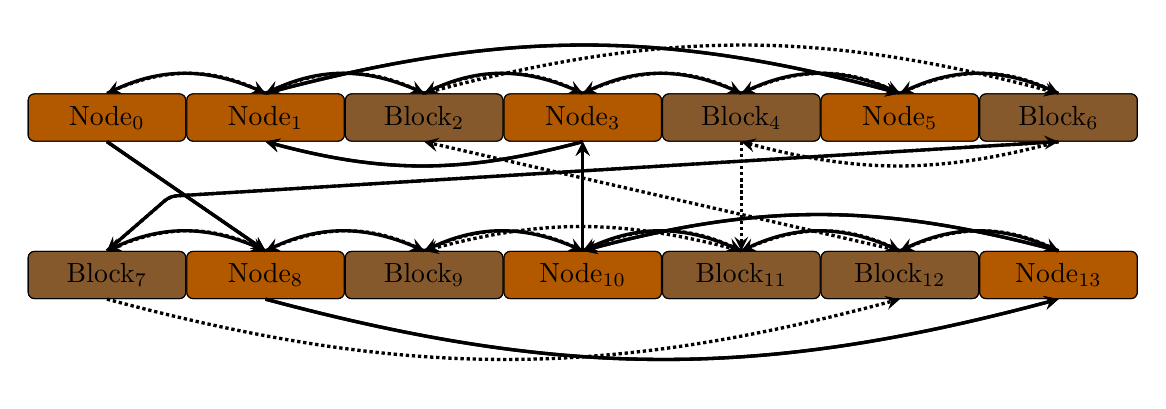
\begin{tikzpicture}[scale=1.0, rounded corners=0.8mm]

   \uncover<1> {
      \mbq (node0)  at (-5.0,4.0) {Block$_0$};
      \mbq (node1)  [right=of node0] {Block$_1$};
      \mbq (node2)  [right=of node1] {Block$_2$};
      \mbq (node3)  [right=of node2] {Block$_3$};
      \mbq (node4)  [right=of node3] {Block$_4$};
      \mbq (node5)  [right=of node4] {Block$_5$};
      \mbq (node6)  [right=of node5] {Block$_6$};

      \mbq (node7)  at (-5.0,2.0)     {Block$_7$};
      \mbq (node8)  [right=of node7] {Block$_8$};
      \mbq (node9)  [right=of node8] {Block$_9$};
      \mbq (node10) [right=of node9] {Block$_{10}$};
      \mbq (node11) [right=of node10] {Block$_{11}$};
      \mbq (node12) [right=of node11] {Block$_{12}$};
      \mbq (node13) [right=of node12] {Block$_{13}$};

      \marrow (node0.north) to [bend right=-25] (node1.north);
      \marrow (node1.north) to [bend right=-25] (node2.north);
      \marrow (node2.north) to [bend right=-25] (node3.north);
      \marrow (node3.north) to [bend right=-25] (node4.north);
      \marrow (node4.north) to [bend right=-25] (node5.north);
      \marrow (node5.north) to [bend right=-25] (node6.north);

      \marrow (node6.south)  -- (-4.2, 3.0) -- (node7.north);
      \marrow (node7.north)  to [bend right=-25] (node8.north);
      \marrow (node8.north)  to [bend right=-25] (node9.north);
      \marrow (node9.north)  to [bend right=-25] (node10.north);
      \marrow (node10.north) to [bend right=-25] (node11.north);
      \marrow (node11.north) to [bend right=-25] (node12.north);
      \marrow (node12.north) to [bend right=-25] (node13.north);
   }

   \uncover<2-> {
      \ebq (node0)  at (-5.0,4.0) {Node$_0$};
      \ebq (node1)  [right=of node0] {Node$_1$};
      \mbq (node2)  [right=of node1] {Block$_2$};
      \ebq (node3)  [right=of node2] {Node$_3$};
      \mbq (node4)  [right=of node3] {Block$_4$};
      \ebq (node5)  [right=of node4] {Node$_5$};
      \mbq (node6)  [right=of node5] {Block$_6$};

      \mbq (node7)  at (-5.0,2.0)     {Block$_7$};
      \ebq (node8)  [right=of node7] {Node$_8$};
      \mbq (node9)  [right=of node8] {Block$_9$};
      \ebq (node10) [right=of node9] {Node$_{10}$};
      \mbq (node11) [right=of node10] {Block$_{11}$};
      \mbq (node12) [right=of node11] {Block$_{12}$};
      \ebq (node13) [right=of node12] {Node$_{13}$};
   }

   \uncover<2> {
      \earrow (node0.south) -- (node8.north);
      \earrow (node1.north) to [bend right=-15] (node5.north);
      \earrow (node3.south) to [bend right=-15] (node1.south);
      \earrow (node8.south) to [bend right=15] (node13.south);
      \earrow (node10.north) -- (node3.south);
      \earrow (node13.north) to [bend right=15] (node10.north);
   }

   \uncover<2> {
      \marrow (node2.north) to [bend right=-15] (node6.north);
      \marrow (node6.south) to [bend right=-15] (node4.south);
      \marrow (node4.south) -- (node11.north);
      \marrow (node11.north) to [bend right=15] (node9.north);
      \marrow (node7.south) to [bend right=15] (node12.south);
      \marrow (node12.north) -- (node2.south);
   }

   \uncover<3> {
      \earrow (node0.south) -- (node8.north);
      \earrow (node1.north) to [bend right=-15] (node5.north);
      \earrow (node3.south) to [bend right=-15] (node1.south);
      \earrow (node8.south) to [bend right=15] (node13.south);
      \earrow (node10.north) -- (node3.south);
      \earrow (node13.north) to [bend right=15] (node10.north);
   }


   \uncover<4> {
      \rearrow (node0.north) to [bend right=-25] (node1.north);
      \rearrow (node1.north) to [bend right=-25] (node2.north);
      \rearrow (node2.north) to [bend right=-25] (node3.north);
      \rearrow (node3.north) to [bend right=-25] (node4.north);
      \rearrow (node4.north) to [bend right=-25] (node5.north);
      \rearrow (node5.north) to [bend right=-25] (node6.north);

      \rearrow (node6.south)  -- (-4.2, 3.0) -- (node7.north);
      \rearrow (node7.north)  to [bend right=-25] (node8.north);
      \rearrow (node8.north)  to [bend right=-25] (node9.north);
      \rearrow (node9.north)  to [bend right=-25] (node10.north);
      \rearrow (node10.north) to [bend right=-25] (node11.north);
      \rearrow (node11.north) to [bend right=-25] (node12.north);
      \rearrow (node12.north) to [bend right=-25] (node13.north);
   }

\end{tikzpicture}

\end{frame}

%____________________________________________________________
\begin{frame}[fragile]
{Benchmark: pointer chasing vs. sequential}
\begin{columns}
\begin{column}{0.47\textwidth}

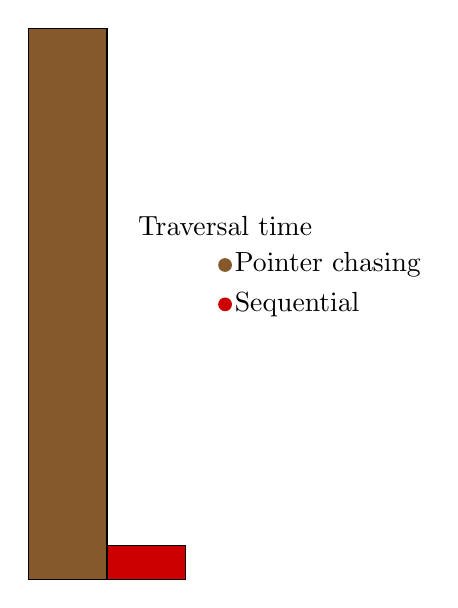
\begin{tikzpicture}[scale=1.0]
\node[anchor=south, draw,node distance=0cm, fill=memC,shape=rectangle,minimum height=7.00cm  ,minimum width=1.0cm]
(node0) at (0cm,0cm) {};
\node[anchor=south,draw,node distance=0cm, fill=alertc,shape=rectangle,minimum height=0.43cm  ,minimum width=1.0cm]
(node1) at (1cm,0.0cm) {};

\node[] at (2cm,4.5cm) {\color{black} Traversal time};
\filldraw[memC] (2cm,4.0cm) circle (0.08cm) node[right]
{\color{black} Pointer chasing};
\filldraw[alertc] (2cm,3.5cm) circle (0.08cm) node[right]
{\color{black} Sequential};

\end{tikzpicture}

\end{column}

\begin{column}{0.47\textwidth}
\begin{block} {Benchmark}
\begin{itemize}
\item Full allocated buffer.
\item Deallocating lots of elements would eventually
make both perform the same.
\end{itemize}
\end{block}
\end{column}
\end{columns}
\end{frame}

%____________________________________________________________
\begin{frame}{Why it is so important to avoid jumping around}{Cache Hierarchy - Speed}
    \begin{columns}
        \begin{column}{0.33\textwidth}

        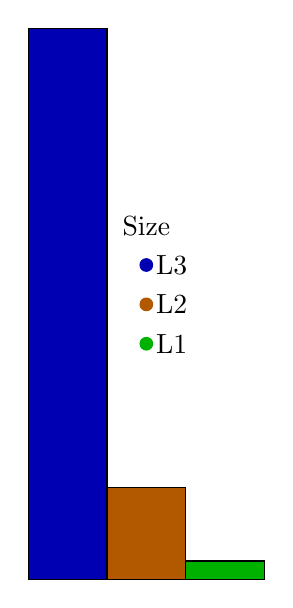
\begin{tikzpicture}[scale=1.0]
        \node[anchor=south, draw,node distance=0cm, fill=nodecontc,shape=rectangle,minimum height=7.0cm  ,minimum width=1.0cm]
        (node0) at (0cm,0cm) {};
        \node[anchor=south,draw,node distance=0cm, fill=bothcontc,shape=rectangle,minimum height=1.17cm  ,minimum width=1.0cm]
        (node1) at (1cm,0.0cm) {};
        \node[anchor=south,draw,node distance=0cm, fill=arraycontc,shape=rectangle,minimum height=0.15cm  ,minimum width=1.0cm]
        (node2) at (2cm,0cm) {};

        \node[] at (1cm,4.5cm) {\color{black} Size};
        \filldraw[nodecontc] (1cm,4.0cm) circle (0.08cm) node[right] {\color{black} L3};
        \filldraw[bothcontc] (1cm,3.5cm) circle (0.08cm) node[right] {\color{black}L2};
        \filldraw[arraycontc] (1cm,3.0cm) circle (0.08cm) node[right] {\color{black}L1};

        \end{tikzpicture}
        \end{column}

        \begin{column}{0.33\textwidth}

        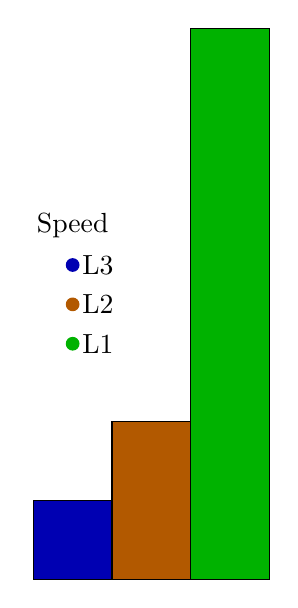
\begin{tikzpicture}[scale=1.0]
        \node[anchor=south, draw,node distance=0cm, fill=nodecontc,shape=rectangle,minimum height=1.00cm  ,minimum width=1.0cm]
        (node0) at (0cm,0cm) {};
        \node[anchor=south,draw,node distance=0cm, fill=bothcontc,shape=rectangle,minimum height=2.00cm  ,minimum width=1.0cm]
        (node1) at (1cm,0.0cm) {};
        \node[anchor=south,draw,node distance=0cm, fill=arraycontc,shape=rectangle,minimum height=7.00cm  ,minimum width=1.0cm]
        (node2) at (2cm,0cm) {};

        \node[] at (0cm,4.5cm) {\color{black} Speed};
        \filldraw[nodecontc] (0cm,4.0cm) circle (0.08cm) node[right] {\color{black} L3};
        \filldraw[bothcontc] (0cm,3.5cm) circle (0.08cm) node[right] {\color{black}L2};
        \filldraw[arraycontc] (0cm,3.0cm) circle (0.08cm) node[right] {\color{black}L1};

        \end{tikzpicture}
        \end{column}

        \begin{column}{0.3\textwidth}
          \begin{block} {Intel Haswell Mobile}
            \begin{itemize}
                \item Register: Fastest
                \item L0: 6 KiB
                \item L1: 128 KiB - 700 GiB/s
                \item L2: 1 MiB - 200 GiB/s
                \item L3: 6 MiB - 100 GB/s
                \item L4: 128 MiB - 40 GB/s
                \item Main memory – GiB - 10 GB/s
            \end{itemize}
          \end{block}
        \end{column}

    \end{columns}
\end{frame}

%____________________________________________________________
\begin{frame}[fragile]
{Alternative to pointer chasing}
{Typical example}
\begin{columns}
\begin{column}{0.47\textwidth}
\begin{lstlisting}
// Allocator configured to chunks of 8
// nodes.
using alloc_type =
    node_allocator<int, node_type, 8>;

std::list<int, alloc_type> l = {1, 2, 3};

auto alloc = l.get_allocator();

const auto n =
    std::count_if( std::begin(alloc)
                 , std::end(alloc),
                 , in_use());
// n = 3
\end{lstlisting}

\end{column}
\begin{column}{0.47\textwidth}
\begin{block} {Code example}
\begin{itemize}
\item Contructor marks the memory block in use.
\item Destructors mark them free.
\item \texttt{std::count\_if} traverses the underlying buffer
ignoring unused nodes.
\end{itemize}
\end{block}
\end{column}
\end{columns}
\end{frame}

\subsection{Reducing the pointer overhead in nodes}

%____________________________________________________________
\begin{frame}[fragile]
{}

\begin{columns}
\begin{column}{0.10\textwidth}
\end{column}
\begin{column}{0.80\textwidth}
\begin{block}{A Flame About 64-bit Pointers}
{ \it \noindent
It is absolutely idiotic to have 64-bit pointers when I compile a
program that uses less than 4 gigabytes of RAM. When such pointer
values appear inside a struct, they not only waste half the memory,
they effectively throw away half of the cache.}  \hfill (Donald Knuth)
\end{block}
\uncover<2> {
\begin{block}{Let us further explore this idea}
\noindent
A node allocator uses a deque-like data structure whose elements
have indexed access. Nodes do not need to store pointers to other
nodes, they can store indexes.
\end{block}
}
\end{column}
\begin{column}{0.10\textwidth}
\end{column}
\end{columns}
\end{frame}


%_____________________________________________________________
\begin{frame}[fragile]
{Pointers are a big overhead on nodes with small sizes}
{Nodes sizes if indexing were possible}
\begin{columns}
\begin{column}{0.5\textwidth}

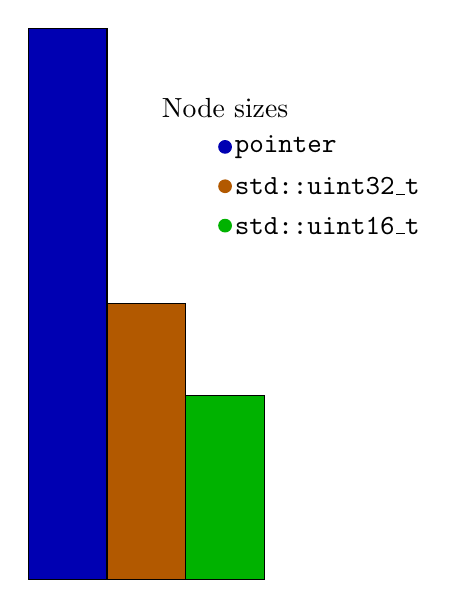
\begin{tikzpicture}[scale=1.0]
\node[anchor=south, draw,node distance=0cm, fill=nodecontc,shape=rectangle,minimum height=7.0cm  ,minimum width=1.0cm]
(node0) at (0cm,0.0cm) {};
\node[anchor=south,draw,node distance=0cm, fill=bothcontc,shape=rectangle,minimum height=3.5cm  ,minimum width=1.0cm]
(node1) at (1cm,0.0cm) {};
\node[anchor=south,draw,node distance=0cm, fill=arraycontc,shape=rectangle,minimum height=2.33cm  ,minimum width=1.0cm]
(node2) at (2cm,0.0cm) {};
%\node[anchor=south,draw,node distance=0cm, fill=purple,shape=rectangle,minimum height=0.875cm  ,minimum width=1.0cm]
%(node3) at (3cm,0.0cm) {};

\node[] at (2cm,6.0cm)
{\color{black} Node sizes};
\filldraw[nodecontc] (2cm,5.5cm) circle (0.08cm) node[right] {\color{black} \texttt{pointer}};
\filldraw[bothcontc] (2cm,5.0cm) circle (0.08cm) node[right] {\color{black} \texttt{std::uint32\_t}};
\filldraw[arraycontc] (2cm,4.5cm) circle (0.08cm) node[right] {\color{black} \texttt{std::uint16\_t}};
%\filldraw[purple] (2cm,4.0cm) circle (0.08cm) node[right] {\color{black} \texttt{std::uint8\_t}};

\end{tikzpicture}

\end{column}
\begin{column}{0.5\textwidth}
\begin{lstlisting}
// Typical node
struct node {
  link_type prev;
  link_type next;
  int info;
};
\end{lstlisting}
\begin{block}{Thoughts}
\begin{itemize}
\item On a 64 bits system the struct size is 24 bytes.
\item Pretty offten bytes by are wasted on padding.
\item Using 32 bits pointers may not be an option.
\item Even if it were, 8 or 16 bits could be enough.
\end{itemize}
\end{block}

\end{column}
\end{columns}

\end{frame}

%_____________________________________________________________
\begin{frame}[fragile]
{Pointers are a big overhead on nodes with small sizes}
{Nodes sizes if indexing were possible}
\begin{columns}
\begin{column}{0.5\textwidth}

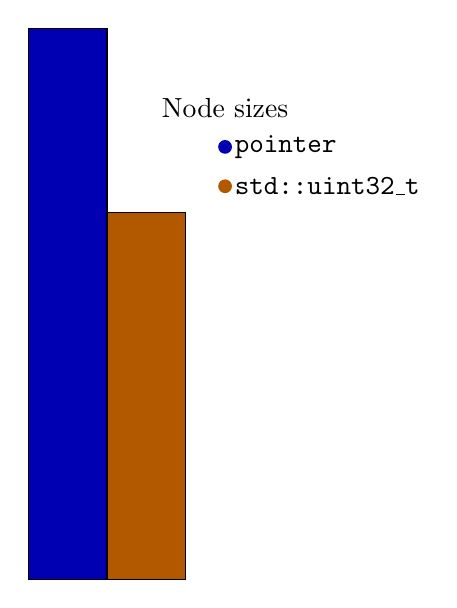
\begin{tikzpicture}[scale=1.0]
\node[anchor=south, draw,node distance=0cm, fill=nodecontc,shape=rectangle,minimum height=7.0cm  ,minimum width=1.0cm]
(node0) at (0cm,0.0cm) {};
\node[anchor=south,draw,node distance=0cm, fill=bothcontc,shape=rectangle,minimum height=4.66cm  ,minimum width=1.0cm]
(node1) at (1cm,0.0cm) {};
%\node[anchor=south,draw,node distance=0cm, fill=arraycontc,shape=rectangle,minimum height=2.33cm  ,minimum width=1.0cm]
%(node2) at (2cm,0.0cm) {};
%\node[anchor=south,draw,node distance=0cm, fill=purple,shape=rectangle,minimum height=0.875cm  ,minimum width=1.0cm]
%(node3) at (3cm,0.0cm) {};

\node[] at (2cm,6.0cm)
{\color{black} Node sizes};
\filldraw[nodecontc] (2cm,5.5cm) circle (0.08cm) node[right] {\color{black} \texttt{pointer}};
\filldraw[bothcontc] (2cm,5.0cm) circle (0.08cm) node[right] {\color{black} \texttt{std::uint32\_t}};
%\filldraw[arraycontc] (2cm,4.5cm) circle (0.08cm) node[right] {\color{black} \texttt{std::uint16\_t}};
%\filldraw[purple] (2cm,4.0cm) circle (0.08cm) node[right] {\color{black} \texttt{std::uint8\_t}};

\end{tikzpicture}

\end{column}
\begin{column}{0.5\textwidth}
\begin{lstlisting}
// Typical node
struct node {
  link_type prev;
  link_type next;
  std::string info;
};
\end{lstlisting}
%\begin{block}{Thoughts}
%\begin{itemize}
%\item Even if it were, 8 or 16 bits could be enough.
%\end{itemize}
%\end{block}

\end{column}
\end{columns}

\end{frame}

%_____________________________________________________________
\begin{frame}[fragile]
{Pointers are a big overhead on nodes with small sizes}
{Nodes sizes if indexing were possible: The extreme case}
\begin{columns}
\begin{column}{0.5\textwidth}

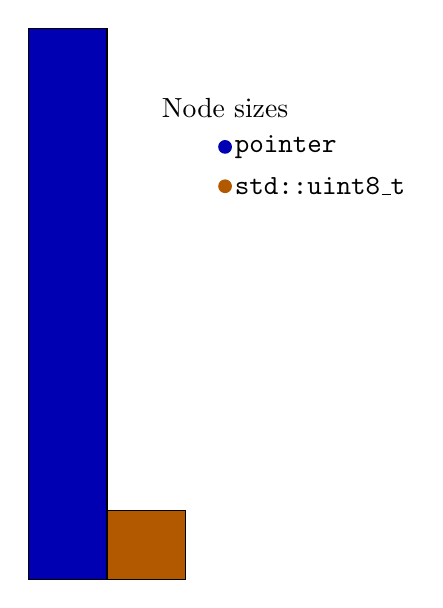
\begin{tikzpicture}[scale=1.0]
\node[anchor=south, draw,node distance=0cm, fill=nodecontc,shape=rectangle,minimum height=7.0cm  ,minimum width=1.0cm]
(node0) at (0cm,0.0cm) {};
\node[anchor=south,draw,node distance=0cm, fill=bothcontc,shape=rectangle,minimum height=0.875cm  ,minimum width=1.0cm]
(node1) at (1cm,0.0cm) {};
%\node[anchor=south,draw,node distance=0cm, fill=arraycontc,shape=rectangle,minimum height=2.33cm  ,minimum width=1.0cm]
%(node2) at (2cm,0.0cm) {};
%\node[anchor=south,draw,node distance=0cm, fill=purple,shape=rectangle,minimum height=0.875cm  ,minimum width=1.0cm]
%(node3) at (3cm,0.0cm) {};

\node[] at (2cm,6.0cm)
{\color{black} Node sizes};
\filldraw[nodecontc] (2cm,5.5cm) circle (0.08cm) node[right] {\color{black} \texttt{pointer}};
\filldraw[bothcontc] (2cm,5.0cm) circle (0.08cm) node[right] {\color{black} \texttt{std::uint8\_t}};
%\filldraw[arraycontc] (2cm,4.5cm) circle (0.08cm) node[right] {\color{black} \texttt{std::uint16\_t}};
%\filldraw[purple] (2cm,4.0cm) circle (0.08cm) node[right] {\color{black} \texttt{std::uint8\_t}};

\end{tikzpicture}

\end{column}
\begin{column}{0.5\textwidth}
\begin{lstlisting}
// Extreme case. Small value type.
// Small number of elements.
struct node {
  link_type prev;
  link_type next;
  unsigned char ages;
};
\end{lstlisting}

\end{column}
\end{columns}

\end{frame}

%____________________________________________________________
%\begin{frame}[fragile]{What if I could address elements with integers}
%\begin{columns}
%\begin{column}{0.5\textwidth}
%
%\begin{tikzpicture}[scale=1.0]
%\node[anchor=south, draw,node distance=0cm, fill=nodecontc,shape=rectangle,minimum height=7.0cm  ,minimum width=1.0cm]
%(node0) at (0cm,0.0cm) {};
%\node[anchor=south,draw,node distance=0cm, fill=bothcontc,shape=rectangle,minimum height=3.5cm  ,minimum width=1.0cm]
%(node1) at (1cm,0.0cm) {};
%\node[anchor=south,draw,node distance=0cm, fill=arraycontc,shape=rectangle,minimum height=1.75cm  ,minimum width=1.0cm]
%(node2) at (2cm,0.0cm) {};
%\node[anchor=south,draw,node distance=0cm, fill=purple,shape=rectangle,minimum height=0.875cm  ,minimum width=1.0cm]
%(node3) at (3cm,0.0cm) {};
%
%\node[] at (2cm,6.0cm) {\color{black} Size in bytes};
%\filldraw[nodecontc] (2cm,5.5cm) circle (0.08cm) node[right] {\color{black} 16};
%\filldraw[bothcontc] (2cm,5.0cm) circle (0.08cm) node[right] {\color{black}8};
%\filldraw[arraycontc] (2cm,4.5cm) circle (0.08cm) node[right] {\color{black}4};
%\filldraw[purple] (2cm,4.0cm) circle (0.08cm) node[right] {\color{black}1};
%
%\end{tikzpicture}
%
%\end{column}
%\begin{column}{0.5\textwidth}
%
%\begin{lstlisting}
%struct node1 {     // sizeof (node2) = 2
%  std::uint8_t n;  // 256 elements.
%  std::uint8_t v;  // [0, 256]
%};
%
%struct node2 {     // sizeof (node2) = 4
%  std::uint16_t n; // 2^16 elements.
%  std::uint16_t v; // [0, 2^16]
%};
%
%struct node3 {     // sizeof (node3) = 8
%  std::uint32_t n; // 2^32 elements.
%  std::uint32_t v; // [0, 2^32]
%};
%
%struct node4 {     // sizeof (node4) = 16
%  node* next;      // Full address space
%  std::size_t v;
%};
%
%\end{lstlisting}
%
%\end{column}
%\end{columns}
%
%\end{frame}

%____________________________________________________________
\begin{frame}
{Speedup due to data locality}
%{}
\begin{columns}

    \begin{column}{0.47\textwidth}
        \begin{center}
            \includegraphics[scale=0.7]{fig/rtset_bench.pdf} \\
        \end{center}
    \end{column}

    \begin{column}{0.47\textwidth}
         \begin{block}{Why so much speed up?}
           \begin{itemize}
           \item Same data structure.
           \item But 4 times more data in the cache.
           \item Uses \texttt{std::uint16\_t} as index
           and \texttt{short} as \texttt{value\_type}
           \item {\color{alertc} Do not forget that 16 bits is
           enough for $65,536$ elements.}
           \end{itemize}
         \end{block}
    \end{column}

\end{columns}
\end{frame}

%____________________________________________________________
\begin{frame}[fragile]
{How to achieve this without breaking code}
{Back to fancy pointers}

\begin{columns}
\begin{column}{0.60\textwidth}
\begin{lstlisting}
template<class Alloc>
struct allocator_traits {
  // Equal to Alloc::link_type if present,
  // Alloc::pointer otherwise. Not required to
  // be a pointer. Nodes store a link and not a
  // pointer.
  using link_type = ...

  // Convert a node link to a pointer.
  pointer make_ptr(link_type a);
};
\end{lstlisting}
\end{column}

\begin{column}{0.40\textwidth}
\begin{block}{Why}
\begin{itemize}
\item Define a fancy pointer that detect when
it is inside a node.
\item Fancy pointer specialization contains
only an index (e.g. \texttt{std::uint16\_t})
\item Function to convert between a \texttt{link\_type}
and \texttt{pointer}.
\item \texttt{link\_type} equal to \texttt{pointer}
in current cases.
\end{itemize}
\end{block}
\end{column}

\end{columns}

\end{frame}

%____________________________________________________________
\begin{frame}[fragile]
{How to achieve this without breaking code}
{Back to fancy pointers}

\begin{columns}
\begin{column}{0.47\textwidth}
\begin{block}{Summary}
\begin{itemize}
\item Incorporate node allocation.
\item Alternative to pointer chasing.
\item Reduce pointer size overhead in nodes.
\item Make STL containers more flexible reduce
the need of new containers to handle corner cases.
\end{itemize}
\end{block}
\end{column}
\begin{column}{0.47\textwidth}
\begin{block}{Acknoledgements}
\begin{itemize}
\item \texttt{std-proposal}
\item \texttt{WG21-SG14}
\item \texttt{ccppbrasil}
\end{itemize}
\end{block}
\end{column}
\end{columns}

\end{frame}

%____________________________________________________________
\begin{frame}{}
    \vspace{1cm}
    \begin{center}
        {\Large \bf Thank you! Questions?} 
    \end{center}
\end{frame}

\end{document}


